\begin{document}


\tikzset{
	axis lines/.style     ={-latex, thick, every node/.style={above}},
	blue line/.style      ={line width=1.1pt, blue!40!black,every node/.style={black}},
	vector/.style          ={line width=1.1pt, -stealth},
	thick vector/.style ={line width=1.5pt, -stealth},
    angle/.style={draw, angle eccentricity=1.5, angle radius=0.5cm, line width=0.7pt}
}

\begin{tikzpicture}[scale=0.75]
	\begin{scope}[axis lines] % Координатные оси
		\draw (-1,0) -- (8,0) node {$t, \text{с}$};
		\draw (0,0) -- (0,3.5) node {$a, \text{м}/\text{с}^2$};
	\end{scope}

	% Подписи
	\draw (0,3) node[left]{60};
    \foreach \t in {0,2,5,9,12} \draw (0.5*\t,0) node[below]{\t};

	\draw[blue line] (-1,0) -- (1,0) -- (2.5,3) -- (4.5,3) -- (6,0) -- (7.5,0);
	\draw[dashed] (0,3) -- (2.5,3) -- (2.5,0)  (4.5,3) -- (4.5,0);
\end{tikzpicture}


\begin{tikzpicture}[scale=1]
	\begin{scope}[axis lines] % Координатные оси
		\draw (0, 0) -- (5,0) node {$t, \text{с}$};
		\draw (0,-2) -- (0,2) node {$v_x, \text{м}/\text{с}$};
	\end{scope}

	\foreach \t in {-10,0,10} \draw (0.12,0.1*\t) --+ (-0.24,0) node[left]{\t};
	\foreach \t in {1,...,5}     \draw (0.35*\t,0.1) --+ (0,-0.2);
	\draw (0.35*5,-0.1) node[below]{5};

	\draw[blue line] (0,-1) -- (3.5,1);
\end{tikzpicture}

\begin{tikzpicture}[scale=0.75]
	\draw[dashed] (-2,0) -- (4,0);
	\begin{scope}[thick vector]
		\draw (0,0)    --+ (2,0)    node[midway, below] {$\vec v$};
		\draw (4,1.5) --+(-1.4,0) node[midway, above] {$\vec u$};
	\end{scope}
	\fill[yellow, draw=black,thick] (4,-2) rectangle (5,2);
	\fill[gray!50, draw=black, thick] (0,0) circle(0.3cm);
\end{tikzpicture}


\begin{tikzpicture}
	\draw[thick] (-1,0) -- (5,0);
	\foreach \x in {-1,-0.9,...,5} \draw (\x+0.075,0) --+ (-0.1,-0.1);
	\draw[line width=1.2pt] (0,0) -- (30:4) |- cycle;
	\path (1.5,0) coordinate (A) (3,0) coordinate (B);
	\draw (0:0.4) arc(0:30:0.4) node[midway,shift={(15:0.4)}] {$\alpha$};

	\begin{scope}[shift={(30:2.4)}, rotate=30, yshift=0.3pt]
		\draw[rounded corners=0.6mm,line width=0.7pt]
			(0,0) -- (0,0.15) -- (0.3,0.15) -- (0.3,0)-- cycle;
		\path (0.15,0.075) coordinate (C);
	\end{scope}
	\draw[vector] (C) -- ($1.5*(A)-0.5*(C)$) node [above left] {$\vec v$};
	\draw pic[pic text={$\beta$},draw, angle eccentricity=1.5, angle radius=0.4cm] {angle=B--A--C};
\end{tikzpicture}\hfill
\begin{tikzpicture}
	\draw[line width=0.7pt] (-3,0) -- (3,0);
	\foreach \x in {-3,-2.9,...,3} \draw (\x+0.075,0) --+ (-0.1,-0.1);
	\draw[line width=1.2pt, latex-latex,scale=1.3]
		(1,0) node[above] {$x$} -- (0,0) --
		(0,1) node[left]  {$y$};
	\path   coordinate (B) node[above left]  {$B$}
	 (0 ,2) coordinate (O) node[left]  {$O$}
	+(60:2) coordinate (A) node[above right] {$A$}
	+(90:2) coordinate (C);
	\fill (O) circle (1.2pt);
	\draw[line width=0.7pt] (C) -- (O) node[midway,left] {$R$} -- (A) -- (B)
		(O) circle (2cm)
		pic[pic text={$\varphi$},draw, angle eccentricity=1.5,
			angle radius=0.5cm] {angle=A--O--C};
	\draw[line width=1pt, -stealth] (O) --+ (1.4,0) node[below] {$v_0$};
\end{tikzpicture}

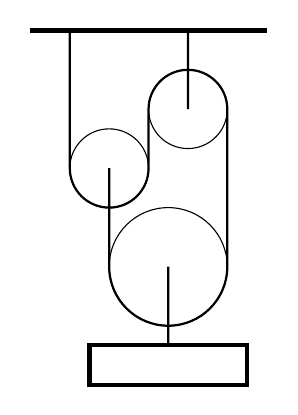
\begin{tikzpicture}[scale=0.5]
	\path 	(-1,-3.5) coordinate (A) +(-1  ,0) coordinate (Al) +(+1  ,0) coordinate (Ar)
			( 1,-2.0) coordinate (B) +(-1  ,0) coordinate (Bl) +(+1  ,0) coordinate (Br)
			(0.5, -6) coordinate (C) +(-1.5,0) coordinate (Cl) +(+1.5,0) coordinate (Cr);
	\draw[line width=2pt] (-3,0) -- (3,0);
	\draw (A) circle (1cm) (B) circle (1cm) (C) circle (1.5cm);
	\draw[thick]
		  (-2,0) -- (Al) arc (180:360:1cm) 	--
					(Bl) arc (180:0:1cm) 	--
					(Cr) arc (0:-180:1.5cm) -- (A)
		  (1,0) -- (B) (C) --+ (0,-2) coordinate (P);
	\draw[shift={(P)},line width=1.5pt] (-2,0) rectangle (2,-1);
\end{tikzpicture}

\begin{tikzpicture}
\draw[line width=1.2pt, latex-latex]
	(4,0) node[above]      {$x$} --
	(0,0) node[below left] {$0$} --
	(0,4) node[right]      {$y$};
\path (3,0)      coordinate (B) node[below]        {$B$}
	  (0,3)      coordinate (A) node[left]         {$A$}
 ($(A)!0.5!(B)$) coordinate (C) node[above right]  {$C$};
\fill (C) circle (0.75mm);
\draw[line width=0.6pt] (A) -- (B);
\draw[line width=1.3pt, -stealth] (A)++(0.1,-0.1) --+ (0,0.7) node[right, midway] {$\vec v$};
\end{tikzpicture}
\vskip1cm

\begin{tikzpicture}
	\draw[thick, latex-latex]
		(4,0) node[above]      {$y$} --
		(0,0) node[below left] {$0$} --
		(0,4) node[right]      {$v(y)$};
	\path 	(3,0)    coordinate (B) node[below] {$2R$}
				(0,3)    coordinate (A) node[left]  {$2v_0$}
         ($(A)+(B)$) coordinate (C);

	\draw[thick] (0,0) -- (C);
	\draw[dashed] (A) -- (C) -- (B);
\end{tikzpicture}

\begin{tikzpicture}
	\path (-3,0.3) coordinate (A) node[above left] {A}
		  ( 3,0.3) coordinate (B) node[above left] {B}
		  (3,-0.3) coordinate (C);
	\draw (A) --+ (0,-1.5) --+ (0,-1.2) coordinate (a)
	      (B) --+ (0,-1.5) --+ (0,-1.2) coordinate (b);
	\draw[dashed] (C)      --+ (1,0)    coordinate (c);
	\draw[latex-latex, thick] (a) -- (b) node[midway,above] {L};

	\begin{scope}
		\clip (A) rectangle (C);
		\foreach \x in {-5,-4.85,...,7} \draw (\x,1) --+ (-2,-2);
	\end{scope}

	\draw[thick] (A) rectangle (C);

	\begin{scope}[vector]
		\draw (A) --+ (30:2.5)  coordinate (Aa) node[right] {$V_A$};
		\draw (C) --+ (-60:1.5) coordinate (Ca) node[right] {$V_B$};
	\end{scope}
	\draw pic[angle, pic text={$\beta$}]  {angle=Ca--C--c}
		       pic[angle, pic text={$\alpha$}] {angle=B--A--Aa};
\end{tikzpicture}

\begin{tikzpicture}
	\path (90:4) coordinate (A) (90:3) coordinate (a) (90:5)   coordinate (AA)
	          (55:4) coordinate (B) (55:3) coordinate (b) (55:5.5) coordinate (BB)
     (B) +(0,-2) coordinate (Bb);
	\draw[line width=0.7pt,dashed] (AA) -- (0,0) -- (BB) (B) -- (Bb);
	\draw[line width=2pt] (a) -- (A)  (b)-- (B);
	\draw[line width=1pt] (A) circle(1cm) (B) circle(1cm);
	\draw pic[	draw, angle radius=0.65cm, line width=0.7pt,-latex] {angle=Bb--B--b}
		(B) node[left] {$\varphi_1$}
		(0.4,1.2) node {$\varphi_2$}
		(1.9,1.7) node {$\varphi_2$};
\end{tikzpicture}

\begin{tikzpicture}
	\draw[thick] (-1.5,0) -- (1.5,0);
	\draw[thick vector] (2.1,2.5) -- +(-1.7,0) node[below] {$\vec V$};
	\draw[thick] (2.1,0) rectangle +(1,3);

	\draw[line width=2.5pt, line cap=rect]         (0,0) -- (2,2);
	\draw[white,line width=1.25pt, line cap=rect] (0,0) -- (2,2);

	\fill (0,0) circle(2.5pt) node[below left] {A};
	\draw (1,0.35) node {$\alpha$};
\end{tikzpicture}

\begin{tikzpicture}
	\path (-1,0) arc (150:90:0.25) coordinate (P);
	\draw (-3,0) -- (-1,0) arc (150:-80:0.25) --+ (0,-2);
	\draw[blue line] (P) + (-1,0) coordinate (F) -- (P) arc (90:-0:0.25)
                                  --+ (0,-1) coordinate (T) --+(0,-2);
	\draw (-0.75,-0.12) node[] {$k$};
	\draw[draw=black, fill=yellow!50] (T)+(0.02,-0.2) rectangle +(0.3,0.3);
	\draw[draw=black, fill=black!30] (F)+(0.02,0.125) rectangle +(-0.4,-0.125);
	\begin{scope}[vector]
		\draw (T)++(0.15,0) --+ (0,-0.6) node[right] {$m\vec g$};
		\draw (F)++(-0.2,0) --+ (0,-1)    node[right] {$M\vec g$};
	\end{scope}
	\begin{scope}[thick, latex-latex]
		\draw (P)++(0.25,0.5) -- +(-1.45,0) node [midway, above]{$L$};
		\draw (-2.5,0.1) -- +(0,-1.2) coordinate (H) node [midway, left]{$H$};
	\end{scope}
	\draw[dashed] (H) --+ (2,0) (-2.5,0.1) --+ (0.4,0) (P)++(0.25,-0.45) --+ (0,1.15) (F)++(-0.2,0.2) --+ (0,0.5);
\end{tikzpicture}

\begin{tikzpicture}[]
	%\draw (-3,0) -- (3,0);
	\path (2,0) coordinate (A);
	\begin{scope}[rotate=20]
		\draw let \p{P} = (A) in (\x{P},0)  coordinate (a)  (0,\y{P}) coordinate (b);
		\draw[gray] let \p{P} = (A) in (A) circle [radius=\y{P}];
		\draw[vector] (0,0) --+ (a) node[above]{$\vec v_{\text{отн}}$};
		\draw[vector,blue line] (A) -- (a) node[midway,right]{$\vec v_{\text{ч}}$};
		\draw[vector,blue line] (0,0) -- (A) node[midway,below]{$-\vec V_{\text{А}}$};
	\end{scope}
	\draw[dashed] (0,0) -- ($3*(a)$) coordinate (Auto) -| cycle (0,0) -- ($-3*(b)$) -| cycle;
	\draw[thick] (Auto)+ (0.1,0) --+ (-6.4,0);
	\draw[vector,blue line] (Auto) --+ (-1,0) node [above]{$\vec V_{\text{А}}$};
	\draw (Auto)+ (-3,0) node[above] {$l_0$}  (0,1) node[right] {$l$}
				(100:1) node {$\alpha$} (10:1) node {$\alpha$};
\end{tikzpicture}

\begin{tikzpicture}[scale=1.75]
	\coordinate (O) at (0,0);
	\coordinate (B) at (40:1);
	\coordinate (A) at (0,3);

	\path let
		\n3 = {0.27cm},
		\p1 = ($(B)-(A)$),
		\n1 = {\n3/\x1},
		\p2 = ($(B)-(O)$),
		\n2 = {\n3/\x2}
		in (-\n1*\x1, -\n1*\y1) coordinate (a)
			( \n2*\x2,  \n2*\y2) coordinate (b)
			($-1*(a)-1*(b)$)      coordinate (c);

	\draw (O) circle (1cm);
	\draw (A) node[above] {$A$}
			-- (B) node[left=1.5mm] {$B$}
					 node[midway,right] {$l$}
            -- (O) node[midway,below] {$R$}
					 node[left] {$O$}
            -- (A) node[midway, left] {$d$};
	\begin{scope}[vector]
		\draw (B) --+ (a) node[right]{$\vec{T}$};
		\draw (B) --+ (b) node[right]{$\vec{N}$};
		\draw (B) --+ (c) node[left]{$m\vec{g}$};
	\end{scope}
\end{tikzpicture}

\begin{tikzpicture}[scale=1.75]
	\coordinate (O) at (0,0);
	\coordinate (B) at (40:1);
	\coordinate (A) at (0,3);

	\path let
		\n3 = {0.27cm},
		\p1 = ($(B)-(A)$),
		\n1 = {\n3/\x1},
		\p2 = ($(B)-(O)$),
		\n2 = {\n3/\x2}
		in (-\n1*\x1, -\n1*\y1) coordinate (a)
			( \n2*\x2,  \n2*\y2) coordinate (b)
			($-1*(a)-1*(b)$)      coordinate (c);

	\shade [ball color= white]  (O) circle (1cm);
	\fill (O) circle (1pt); \fill (A) circle (1pt);
	\draw (A) node[above] {$A$}  -- ($1.1*(B)$) node[midway,right] {$l$};
	\shade [ball color= gray]  ($1.1*(B)$) circle [radius=0.1cm];
    \draw (O)  node[left] {$O$}  -- (A) node[midway, left] {$d$};
\end{tikzpicture}

\begin{tikzpicture}[scale=1.75]
	\coordinate (O) at (0,0);
	\coordinate (B) at (40:1);
	\coordinate (A) at (0,3);

	\path let
		\n3 = {0.27cm},
		\p1 = ($(B)-(A)$),
		\n1 = {\n3/\x1},
		\p2 = ($(B)-(O)$),
		\n2 = {\n3/\x2}
		in (-\n1*\x1, -\n1*\y1) coordinate (a)
			( \n2*\x2,  \n2*\y2) coordinate (b)
			($-1*(a)-1*(b)$)      coordinate (c);


	\begin{scope}[vector]
		\draw (0,0) --+ (b) node[right]{$\vec{N}$};
		\draw (b) --+ (a) node[right]{$\vec{T}$};
		\draw (a)++(b) --+ (c) node[midway,left]{$m\vec{g}$};
	\end{scope}
\end{tikzpicture}

\begin{tikzpicture}[scale=1.75,vector, every node/.style=midway]
		\draw (1,0)    -- (0,0) node[below]{$m\vec{a}$};
		\draw (0,2.15) -- (0,0) node[left]{$m\vec{g}$};
		\draw (1,0) -- (0,2.15) node[right]{$\vec{T}'$};;
\end{tikzpicture}

\end{document}
